% main.tex - HCEA paper skeleton (SCI Q2 target)
% Compile: pdflatex (IEEEtran.cls required; if unavailable, replace
% \documentclass[journal]{IEEEtran} with \documentclass[10pt,twocolumn]{article}
% and delete the IEEEtran-specific commands marked with % IEEEtran).
\documentclass[journal]{IEEEtran}

\usepackage{graphicx}
\usepackage{booktabs}
\usepackage{amsmath,amssymb}
\usepackage{subfig}
\usepackage{cite}
\usepackage[colorlinks=true,linkcolor=blue,citecolor=blue,urlcolor=blue]{hyperref}

\begin{document}

\title{Hypervolume-Verified Dual-Mechanism Switching for Multiobjective Optimization: A Study of IGD--HV Ranking Disagreement on Convex, Concave, and Disconnected Fronts}

\author{[TODO: Author names],~\IEEEmembership{[TODO: affiliations]}% IEEEtran
\thanks{[TODO: corresponding author, funding, acknowledgments]}}

\markboth{[TODO: Journal short title]}% IEEEtran
{[TODO: Authors short form]}% IEEEtran

\maketitle

\begin{abstract}
Indicator-based evaluation dominates the empirical assessment of multiobjective evolutionary algorithms (MOEAs), yet the inverted generational distance (IGD) and the hypervolume (HV) do not always rank algorithms consistently. This paper makes two contributions. First, we quantify this ranking disagreement in a controlled setting: nine algorithms (NSGA-II, NSGA-III, MOEA/D, SPEA2, SMS-EMOA, RVEA, AGE-MOEA, MOGWO, and our proposed HCEA) are run with 30 independent seeds on five bi-objective benchmarks spanning convex (ZDT1), concave (ZDT2, DTLZ2), and disconnected (ZDT3, DTLZ7) fronts. On the four convex/disconnected problems the Spearman correlation between IGD-based and HV-based rankings is $\rho \geq 0.98$; on the concave DTLZ2 it drops to $\rho = 0.57$. A follow-up experiment replacing the reference front with an arc-uniform sampling raises $\rho$ only to $0.63$, showing that the divergence stems from the concave geometry itself (HV-optimal spacing is not arc-uniform), not from reference-front discretization. Second, we propose HCEA, a hybrid algorithm whose environmental-selection mechanism---reference-vector-guided APD selection versus SMS-EMOA-style incremental hypervolume refinement---is switched online at fixed checkpoints, with the switch accepted only when a one-generation trial measurably improves the hypervolume. Across the five problems HCEA attains Friedman mean ranks of 1.8 (HV, second) and 2.8 (IGD, third), is the best algorithm on the disconnected ZDT3 in both metrics, and is statistically indistinguishable from SMS-EMOA and SPEA2 on most problems under the Nemenyi post-hoc test (CD = 5.37 with five blocks). On DTLZ2 its IGD rank is only sixth, an honest weakness we analyze in depth. The study underscores that conclusions about an algorithm's standing are indicator-dependent on concave fronts.
\end{abstract}

\begin{IEEEkeywords}% IEEEtran
Multiobjective optimization, hypervolume, inverted generational distance, indicator disagreement, evolutionary algorithm.% IEEEtran
\end{IEEEkeywords}% IEEEtran

\section{Introduction}
\IEEEPARstart{}{} % IEEEtran (drop-in first character)

Performance evaluation in multiobjective optimization relies on quality indicators, and two of them dominate the literature: the inverted generational distance (IGD), which measures how well a solution set covers a reference Pareto front, and the hypervolume (HV), which measures the volume dominated by the set. IGD rewards solutions whose spacing matches the reference front, whereas HV rewards spacing that maximizes dominated volume, and the two criteria do not always coincide~\cite{zitzler2003performance}. On concave fronts this mismatch is structural: HV-optimal point placements on a quarter circle are not arc-uniform, so an HV-optimal set can be suboptimal in IGD and vice versa.

Our study quantifies this phenomenon and connects it to algorithm design. We evaluate nine algorithms---eight widely used baselines (NSGA-II, NSGA-III, MOEA/D, SPEA2, SMS-EMOA, RVEA, AGE-MOEA, MOGWO) and our proposed HCEA---on five bi-objective benchmarks (ZDT1, ZDT2, ZDT3, DTLZ2, DTLZ7) with 30 independent seeds each. Two findings stand out. First, on the four convex and disconnected problems the IGD-based and HV-based algorithm rankings are almost identical (Spearman $\rho \geq 0.98$), but on the concave DTLZ2 the correlation drops to $\rho = 0.57$: SMS-EMOA and HCEA rank first and second by HV yet only fifth and sixth by IGD, while MOEA/D ranks first by IGD but fourth by HV. Second, this disagreement is not an artifact of the reference-front discretization: recomputing IGD against an arc-uniform reference front changes the correlation only marginally ($\rho = 0.63$). The disagreement is therefore a property of the concave geometry, and it has direct consequences for how reported rankings should be interpreted.

The second contribution is the algorithm HCEA (Hybrid Convergence-Environmental Archive). HCEA alternates between two environmental-selection mechanisms: a reference-vector-guided APD (angle-penalized distance) selection that drives convergence, and an SMS-EMOA-style incremental hypervolume reduction that refines distribution. The switch between the two mechanisms is adjudicated online: at the 50\%, 60\%, and 70\% generation checkpoints, HCEA runs a one-generation trial of the hypervolume mechanism and keeps it only if the measured hypervolume of the population strictly improves. This design makes the switch indicator-aware rather than schedule-based. HCEA is competitive but we report its standing honestly: it achieves the best result on the disconnected ZDT3 in both metrics, Friedman mean ranks of 1.8 (HV) and 2.8 (IGD) over five problems, and it is statistically indistinguishable from SMS-EMOA and SPEA2 on most problems under the Nemenyi test with five blocks (CD = 5.37); on DTLZ2 its IGD rank is sixth, a weakness rooted in the same concave-front geometry that produces the indicator disagreement.

The remainder of the paper is organized as follows. Section~II reviews related work. Section~III describes HCEA. Section~IV details the experimental setup. Section~V reports the results, Section~VI discusses the indicator-disagreement findings and limitations, and Section~VII concludes.

\section{Related Work}
\subsection{Baseline algorithms}
The eight baselines span the main design families in multiobjective optimization: Pareto-dominance-based selection (NSGA-II~\cite{deb2002nsga2}, SPEA2~\cite{zitzler2001spea2}), decomposition (MOEA/D~\cite{zhang2007moead}), reference-vector-guided selection (NSGA-III~\cite{deb2014nsga3}, RVEA~\cite{cheng2016rvea}), indicator-based selection (SMS-EMOA~\cite{beume2007smsemoa}), geometric estimation (AGE-MOEA), and swarm metaheuristics (MOGWO~\cite{mirjalili2016mogwo}). [TODO: one paragraph per family with 2--3 citations each; verify exact bibliographic data.]

\subsection{Multi-stage, dual-archive, and adaptive operator selection}
Several recent works organize the search into stages or archives---e.g., two-archive algorithms and multi-stage many-objective EAs---and adaptive operator selection (AOS) methods such as the fitness-rate-rank multi-armed bandit (FRRMAB)~\cite{li2014frrmab} select variation operators online. HCEA differs from these in two respects: it switches between environmental-selection mechanisms (not variation operators), and the switch decision is adjudicated by a direct measurement of hypervolume improvement rather than accumulated credit. [TODO: cite two-stage/dual-archive representatives (e.g., two-stage two-archive TEVC 2024; multi-stage MaOEA Information Sciences 2021) and a finite-state-machine multi-stage EA (SWEVO 2025); verify DOIs.]

\subsection{Indicator disagreement}
The fact that different indicators can rank the same algorithm set differently is well known~\cite{zitzler2003performance}, but systematic empirical quantification on controlled front geometries remains thin. Our study contributes a five-problem, nine-algorithm, 30-seed measurement and an explicit test (reference-front replacement) that localizes the cause of the disagreement to concave geometry. [TODO: add recent references on indicator choice and benchmarking practice.]

\section{Proposed Algorithm: HCEA}
HCEA maintains a single population of $N$ individuals and one of two environmental-selection mechanisms at any time. In mechanism A (convergence phase), $N$ offspring are generated by SBX and polynomial mutation from a random mating pool, and each static reference vector (generated once by the NBI method) retains the solution with the smallest angle-penalized distance $\mathrm{APD}=(1+M\theta d_i/\gamma_i)\cdot\|f-z^{\ast}\|$, with $\theta=(g/G)^{2}$ annealing the angular term; vacant vectors are refilled by the best-remaining APD so that the population size stays constant. In mechanism B (distribution phase), the algorithm iterates $N$ times: one offspring is generated from two random parents and merged into the population, and the solution with the smallest hypervolume contribution on the last non-dominated front is removed (boundary solutions have infinite contribution and are never deleted), following SMS-EMOA. The switching rule is the core of HCEA: at generations $0.5G$, $0.6G$, and $0.7G$, if mechanism A is active, HCEA runs one full generation of mechanism B on the current population and permanently adopts it if and only if the exact two-dimensional hypervolume (reference point $1.1\times\max$ of the population) strictly increases; otherwise mechanism A remains and the check is retried at the next checkpoint. A light-weight polishing operator (last 10\% of generations) perturbs the lowest-contribution solution a bounded number of times and keeps the best variant. All extra evaluations are counted in the reported nFE. [TODO: add pseudocode (Algorithm~1) and a runtime-complexity paragraph.]

\section{Experimental Setup}
Five bi-objective instances are used (Table~\ref{tab:datasets}): ZDT1 (convex), ZDT2 (concave), ZDT3 (disconnected), DTLZ2 (concave), and DTLZ7 (disconnected). All nine algorithms run with population size $N=100$ for 200 generations; MOGWO keeps the baseline protocol of 500 generations. Each algorithm--problem pair is repeated with seeds 1--30. IGD is computed against the true Pareto front sampled at 500 points; HV is computed exactly in two dimensions with the per-problem reference point $\mathrm{ref} = 1.1 \times \max(\mathrm{PF})$, identical for all algorithms. [TODO: hardware/OS/MATLAB version; note the DTLZ2 ParetoFront uses PlatEMO's NBI discretization while the arc-uniform replacement was used only in the follow-up analysis.]

\section{Results}
\subsection{Overall performance}
Tables~\ref{tab:igd} and~\ref{tab:hv} report the mean and standard deviation of IGD and HV over 30 seeds. [TODO: expand the per-problem narrative, e.g., SMS-EMOA is the best on ZDT1 in IGD ($0.00364$) while HCEA is second ($0.00375$); on DTLZ2 MOEA/D achieves the best IGD ($0.00396$) but only the fourth-best HV ($0.41999$).] Table~\ref{tab:ranks} condenses both metrics into per-problem ranks. On the disconnected ZDT3, HCEA ranks first in both IGD and HV; on DTLZ2 it ranks sixth by IGD but second by HV---the largest single-algorithm divergence observed (rank difference $+4$).

\begin{table}[t]
\centering
\caption{Mean IGD ($\pm$ std) over 30 independent runs; the best value in each column is in bold.}
\label{tab:igd}
\footnotesize
\begin{tabular}{lcccccccc}
\toprule
Algorithm & ZDT1 & ZDT2 & ZDT3 & DTLZ2 & DTLZ7 & DTLZ1\,M3 & DTLZ2\,M3 & DTLZ7\,M3 \\
\midrule
NSGA2 & $0.0051 \pm 2.1e{-4}$ & $0.0051 \pm 1.9e{-4}$ & $0.0074 \pm 7.6e{-3}$ & $0.0051 \pm 1.6e{-4}$ & $0.0053 \pm 1.8e{-4}$ & $0.8670 \pm 6.0e{-1}$ & $0.0701 \pm 2.8e{-3}$ & $0.1129 \pm 9.7e{-2}$ \\
NSGA3 & $0.0293 \pm 2.3e{-2}$ & $0.0253 \pm 2.0e{-2}$ & $0.0434 \pm 3.3e{-2}$ & $0.0289 \pm 1.3e{-2}$ & $0.0218 \pm 1.8e{-2}$ & $1.4806 \pm 1.2e{0}$ & $0.1399 \pm 4.0e{-2}$ & $0.1650 \pm 1.1e{-1}$ \\
MOEAD & $0.0238 \pm 1.8e{-2}$ & $0.1383 \pm 1.1e{-1}$ & $0.0509 \pm 2.7e{-2}$ & \textbf{$0.0040 \pm 2.1e{-6}$} & $0.2276 \pm 2.2e{-1}$ & $1.6215 \pm 1.6e{0}$ & $0.0527 \pm 1.6e{-5}$ & $0.1607 \pm 1.2e{-1}$ \\
SPEA2 & $0.0043 \pm 1.7e{-4}$ & $0.0045 \pm 1.9e{-4}$ & $0.0049 \pm 2.1e{-4}$ & $0.0042 \pm 5.0e{-5}$ & $0.0048 \pm 7.2e{-5}$ & $0.7032 \pm 4.6e{-1}$ & $0.0534 \pm 4.8e{-4}$ & $0.0589 \pm 1.3e{-3}$ \\
SMSEMOA & \textbf{$0.0036 \pm 2.6e{-5}$} & \textbf{$0.0044 \pm 1.3e{-4}$} & $0.0053 \pm 5.5e{-3}$ & $0.0057 \pm 2.2e{-4}$ & \textbf{$0.0042 \pm 2.0e{-5}$} & $1.1694 \pm 8.1e{-1}$ & $0.1009 \pm 1.2e{-2}$ & $0.2079 \pm 1.5e{-1}$ \\
RVEA & $0.0387 \pm 5.4e{-3}$ & $0.0521 \pm 6.8e{-3}$ & $0.0708 \pm 1.8e{-2}$ & $0.0047 \pm 5.6e{-4}$ & $0.0197 \pm 3.9e{-3}$ & $1.2503 \pm 7.0e{-1}$ & \textbf{$0.0527 \pm 3.1e{-5}$} & $0.1070 \pm 4.4e{-3}$ \\
AGEMOEA & $0.0167 \pm 5.8e{-3}$ & $0.0177 \pm 6.4e{-3}$ & $0.0186 \pm 9.3e{-3}$ & $0.0238 \pm 1.1e{-2}$ & $0.0497 \pm 1.1e{-1}$ & $1.1023 \pm 7.7e{-1}$ & $0.1162 \pm 1.6e{-2}$ & $0.2498 \pm 1.6e{-1}$ \\
MOGWO & $0.5336 \pm 2.1e{-1}$ & $0.6057 \pm 1.7e{-2}$ & $0.5556 \pm 1.9e{-1}$ & $0.0759 \pm 2.6e{-2}$ & $0.7781 \pm 6.5e{-2}$ & $71.0324 \pm 2.1e{1}$ & $0.4278 \pm 5.2e{-2}$ & $1.5018 \pm 7.9e{-2}$ \\
HCEA & $0.0037 \pm 3.2e{-5}$ & $0.0045 \pm 1.6e{-4}$ & \textbf{$0.0044 \pm 2.7e{-4}$} & $0.0057 \pm 2.0e{-4}$ & $0.0043 \pm 2.6e{-5}$ & $1.7132 \pm 1.1e{0}$ & $0.0928 \pm 1.7e{-2}$ & $0.1719 \pm 1.7e{-2}$ \\
\bottomrule
\end{tabular}
\end{table}

\begin{table}[t]
\centering
\caption{Mean hypervolume ($\pm$ std) over 30 independent runs; the best value in each column is in bold.}
\label{tab:hv}
\footnotesize
\begin{tabular}{lcccccccc}
\toprule
Algorithm & ZDT1 & ZDT2 & ZDT3 & DTLZ2 & DTLZ7 & DTLZ1\,M3 & DTLZ2\,M3 & DTLZ7\,M3 \\
\midrule
NSGA2 & $0.8689 \pm 4.5e{-4}$ & $0.5356 \pm 4.7e{-4}$ & $1.0193 \pm 8.0e{-3}$ & $0.4193 \pm 2.2e{-4}$ & $1.0097 \pm 1.6e{-4}$ & $0.0016 \pm 2.6e{-3}$ & $0.0634 \pm 5.8e{-3}$ & $0.0882 \pm 2.2e{-2}$ \\
NSGA3 & $0.8429 \pm 1.8e{-2}$ & $0.5035 \pm 2.7e{-2}$ & $0.9686 \pm 4.0e{-2}$ & $0.3886 \pm 1.3e{-2}$ & $0.9830 \pm 3.1e{-2}$ & $0.0008 \pm 1.9e{-3}$ & $0.0581 \pm 1.4e{-2}$ & $0.1238 \pm 7.8e{-2}$ \\
MOEAD & $0.8447 \pm 1.6e{-2}$ & $0.3714 \pm 9.9e{-2}$ & $0.9317 \pm 3.6e{-2}$ & $0.4200 \pm 3.1e{-5}$ & $0.8649 \pm 1.4e{-1}$ & $0.0011 \pm 2.2e{-3}$ & $0.0599 \pm 3.0e{-3}$ & $0.3023 \pm 5.4e{-2}$ \\
SPEA2 & $0.8698 \pm 5.1e{-4}$ & $0.5360 \pm 5.8e{-4}$ & $1.0209 \pm 6.4e{-4}$ & $0.4201 \pm 1.3e{-4}$ & $1.0103 \pm 6.3e{-5}$ & \textbf{$0.0033 \pm 6.8e{-3}$} & $0.0588 \pm 2.6e{-3}$ & $0.1189 \pm 8.4e{-3}$ \\
SMSEMOA & \textbf{$0.8719 \pm 6.2e{-5}$} & \textbf{$0.5386 \pm 6.2e{-5}$} & $1.0226 \pm 5.8e{-3}$ & \textbf{$0.4210 \pm 8.2e{-6}$} & \textbf{$1.0108 \pm 7.0e{-6}$} & $0.0011 \pm 3.1e{-3}$ & $0.0725 \pm 1.2e{-2}$ & $0.1007 \pm 4.2e{-2}$ \\
RVEA & $0.8108 \pm 9.1e{-3}$ & $0.4479 \pm 1.2e{-2}$ & $0.8823 \pm 3.1e{-2}$ & $0.4182 \pm 1.2e{-3}$ & $0.9731 \pm 9.7e{-3}$ & $0.0009 \pm 3.6e{-3}$ & $0.0617 \pm 2.2e{-3}$ & $0.1665 \pm 8.0e{-3}$ \\
AGEMOEA & $0.8533 \pm 7.1e{-3}$ & $0.5239 \pm 3.5e{-3}$ & $1.0005 \pm 1.1e{-2}$ & $0.4069 \pm 6.6e{-3}$ & $0.9624 \pm 6.7e{-2}$ & $0.0020 \pm 5.2e{-3}$ & \textbf{$0.0773 \pm 2.1e{-2}$} & $0.0889 \pm 5.4e{-2}$ \\
MOGWO & $0.3848 \pm 1.8e{-1}$ & $0.1101 \pm 1.0e{-3}$ & $0.3866 \pm 2.1e{-1}$ & $0.3491 \pm 1.7e{-2}$ & $0.4022 \pm 5.4e{-2}$ & $0.0000 \pm 0.0$ & $0.0270 \pm 1.3e{-2}$ & $0.0014 \pm 2.4e{-3}$ \\
HCEA & $0.8716 \pm 1.3e{-4}$ & $0.5381 \pm 2.2e{-4}$ & \textbf{$1.0227 \pm 3.0e{-4}$} & $0.4209 \pm 1.1e{-5}$ & $1.0108 \pm 1.1e{-5}$ & $0.0005 \pm 2.1e{-3}$ & $0.0656 \pm 1.2e{-2}$ & \textbf{$0.3675 \pm 6.6e{-2}$} \\
\bottomrule
\end{tabular}
\end{table}

\begin{table}[t]
\centering
\caption{Per-problem ranks by mean IGD (smaller is better) and mean HV (larger is better), with the average ranks over the eight problems.}
\label{tab:ranks}
\footnotesize
\setlength{\tabcolsep}{2.5pt}
\begin{tabular}{l@{\hspace{3pt}}cc@{\hspace{4pt}}cc@{\hspace{4pt}}cc@{\hspace{4pt}}cc@{\hspace{4pt}}cc@{\hspace{4pt}}cc@{\hspace{4pt}}cc@{\hspace{4pt}}cc@{\hspace{4pt}}cc}
\toprule
 & \multicolumn{2}{c}{ZDT1} & \multicolumn{2}{c}{ZDT2} & \multicolumn{2}{c}{ZDT3} & \multicolumn{2}{c}{DTLZ2} & \multicolumn{2}{c}{DTLZ7} & \multicolumn{2}{c}{DTLZ1\,M3} & \multicolumn{2}{c}{DTLZ2\,M3} & \multicolumn{2}{c}{DTLZ7\,M3} \\
 Algorithm & IGD & HV & IGD & HV & IGD & HV & IGD & HV & IGD & HV & IGD & HV & IGD & HV & IGD & HV \\
\midrule
NSGA2   & 4 & 4 & 4 & 4 & 4 & 4 & 4 & 5 & 4 & 4 & 2 & 3 & 4 & 4 & 3 & 8 & 3.6 & 4.5 \\
NSGA3   & 7 & 7 & 6 & 6 & 6 & 6 & 8 & 8 & 6 & 5 & 6 & 7 & 8 & 8 & 5 & 4 & 6.5 & 6.4 \\
MOEAD   & 6 & 6 & 8 & 8 & 7 & 7 & 1 & 4 & 8 & 8 & 7 & 5 & 1 & 6 & 4 & 2 & 5.3 & 5.8 \\
SPEA2   & 3 & 3 & 2 & 3 & 2 & 3 & 2 & 3 & 3 & 3 & 1 & 1 & 3 & 7 & 1 & 5 & 2.1 & 3.5 \\
SMSEMOA & 1 & 1 & 1 & 1 & 3 & 2 & 5 & 1 & 1 & 1 & 4 & 4 & 6 & 2 & 7 & 6 & 3.5 & 2.3 \\
RVEA    & 8 & 8 & 7 & 7 & 8 & 8 & 3 & 6 & 5 & 6 & 5 & 6 & 2 & 5 & 2 & 3 & 5.0 & 6.1 \\
AGEMOEA & 5 & 5 & 5 & 5 & 5 & 5 & 7 & 7 & 7 & 7 & 3 & 2 & 7 & 1 & 8 & 7 & 5.9 & 4.9 \\
MOGWO   & 9 & 9 & 9 & 9 & 9 & 9 & 9 & 9 & 9 & 9 & 9 & 9 & 9 & 9 & 9 & 9 & 9.0 & 9.0 \\
HCEA    & 2 & 2 & 3 & 2 & 1 & 1 & 6 & 2 & 2 & 2 & 8 & 8 & 5 & 3 & 6 & 1 & 4.1 & 2.6 \\
\bottomrule
\end{tabular}
\end{table}


\subsection{Statistical analysis}
The Friedman test confirms significant overall differences for both metrics (Table~\ref{tab:friedman}): IGD $\chi^2=28.05$, $p=4.64\times10^{-4}$; HV $\chi^2=36.32$, $p=1.53\times10^{-5}$. HCEA's Friedman mean ranks are 2.8 (IGD, third) and 1.8 (HV, second). Pairwise two-sided Wilcoxon tests with 30 seeds per problem (Table~\ref{tab:wilcoxon_igd}) show that HCEA differs significantly from the baselines on most problems, with notable exceptions where it does not: against SPEA2 on ZDT2 ($p=0.186$) and against SMS-EMOA on ZDT3 ($p=0.068$) and DTLZ2 ($p=0.888$). The Nemenyi post-hoc test (Fig.~\ref{fig:cd}) with five blocks gives CD = 5.37, which spans almost the entire rank axis: at $\alpha=0.05$ only MOGWO is separated from the top group in either metric; the fine ordering within the top group (HCEA vs. SMS-EMOA vs. SPEA2) is not statistically supported. [TODO: full per-pair CD statement.]

\begin{table}[t]
\centering
\caption{Friedman mean ranks over the eight problems ($1$ = best).}
\label{tab:friedman}
\begin{tabular}{lcc}
\toprule
Algorithm & IGD rank & HV rank \\
\midrule
NSGA2 & 3.6 & 4.5 \\
NSGA3 & 6.5 & 6.4 \\
MOEAD & 5.3 & 5.8 \\
SPEA2 & 2.1 & 3.5 \\
SMSEMOA & 3.5 & 2.3 \\
RVEA & 5.0 & 6.1 \\
AGEMOEA & 5.9 & 4.9 \\
MOGWO & 9.0 & 9.0 \\
HCEA & 4.1 & 2.6 \\
\midrule
\multicolumn{3}{l}{\footnotesize Note: IGD $\chi^2=34.40$, $p=3.44\times10^{-5}$; HV $\chi^2=37.80$, $p=8.20\times10^{-6}$; df = 8.}\\
\bottomrule
\end{tabular}
\end{table}

\begin{table}[t]
\centering
\caption{Two-sided Wilcoxon rank-sum tests (30 seeds per problem) comparing HCEA with the eight baseline algorithms on IGD: per-problem $p$-values and the Fisher-combined $p$-value over the eight problems.}
\label{tab:wilcoxon_igd}
\footnotesize
\setlength{\tabcolsep}{3pt}
\begin{tabular}{lcccccccc|cl}
\toprule
vs\,HCEA & ZDT1 & ZDT2 & ZDT3 & DTLZ2 & DTLZ7 & DTLZ1\,M3 & DTLZ2\,M3 & DTLZ7\,M3 & Fisher combined & Sig.\\
\midrule
NSGA2 & $3.0\times10^{-11}$ & $8.2\times10^{-11}$ & $3.0\times10^{-11}$ & $3.3\times10^{-11}$ & $3.0\times10^{-11}$ & $2.7\times10^{-4}$ & $1.1\times10^{-6}$ & $1.1\times10^{-6}$ & $<10^{-60}$ & $^{***}$ \\
NSGA3 & $3.0\times10^{-11}$ & $3.0\times10^{-11}$ & $3.0\times10^{-11}$ & $3.0\times10^{-11}$ & $3.0\times10^{-11}$ & $0.25$ (ns) & $2.6\times10^{-7}$ & $3.8\times10^{-3}$ & $<10^{-50}$ & $^{***}$ \\
MOEAD & $3.0\times10^{-11}$ & $3.0\times10^{-11}$ & $3.0\times10^{-11}$ & $3.0\times10^{-11}$ & $3.0\times10^{-11}$ & $0.16$ (ns) & $3.0\times10^{-11}$ & $7.8\times10^{-9}$ & $<10^{-60}$ & $^{***}$ \\
SPEA2 & $3.0\times10^{-11}$ & $0.19$ (ns) & $3.2\times10^{-9}$ & $3.0\times10^{-11}$ & $3.0\times10^{-11}$ & $1.7\times10^{-5}$ & $5.5\times10^{-8}$ & $3.0\times10^{-11}$ & $<10^{-50}$ & $^{***}$ \\
SMSEMOA & $8.2\times10^{-11}$ & $1.7\times10^{-4}$ & $0.07$ (ns) & $0.89$ (ns) & $6.7\times10^{-11}$ & $2.8\times10^{-2}$ & $0.35$ (ns) & $0.09$ (ns) & $1.1\times10^{-24}$ & $^{***}$ \\
RVEA & $3.0\times10^{-11}$ & $3.0\times10^{-11}$ & $3.0\times10^{-11}$ & $4.2\times10^{-9}$ & $3.0\times10^{-11}$ & $0.07$ (ns) & $3.0\times10^{-11}$ & $9.9\times10^{-11}$ & $<10^{-60}$ & $^{***}$ \\
AGEMOEA & $3.0\times10^{-11}$ & $3.0\times10^{-11}$ & $3.0\times10^{-11}$ & $3.0\times10^{-11}$ & $3.0\times10^{-11}$ & $1.1\times10^{-2}$ & $1.4\times10^{-6}$ & $0.50$ (ns) & $<10^{-50}$ & $^{***}$ \\
MOGWO & $3.0\times10^{-11}$ & $4.1\times10^{-12}$ & $3.0\times10^{-11}$ & $3.0\times10^{-11}$ & $2.1\times10^{-11}$ & $3.0\times10^{-11}$ & $3.0\times10^{-11}$ & $2.9\times10^{-11}$ & $<10^{-70}$ & $^{***}$ \\
\midrule
\multicolumn{11}{l}{\footnotesize Significance: $^{*}p<0.05$, $^{**}p<0.01$, $^{***}p<0.001$, ns = not significant. Fisher combined with numerical guard ($\max(p,10^{-300})$); values below $10^{-60}$ shown as $<10^{-60}$.}\\
\bottomrule
\end{tabular}
\end{table}

\begin{table}[t]
\centering
\caption{Two-sided Wilcoxon rank-sum tests (30 seeds per problem) comparing HCEA with the eight baseline algorithms on HV: per-problem $p$-values and the Fisher-combined $p$-value over the eight problems.}
\label{tab:wilcoxon_hv}
\footnotesize
\setlength{\tabcolsep}{3pt}
\begin{tabular}{lcccccccc|cl}
\toprule
vs\,HCEA & ZDT1 & ZDT2 & ZDT3 & DTLZ2 & DTLZ7 & DTLZ1\,M3 & DTLZ2\,M3 & DTLZ7\,M3 & Fisher combined & Sig.\\
\midrule
NSGA2 & $3.0\times10^{-11}$ & $3.0\times10^{-11}$ & $3.0\times10^{-11}$ & $3.0\times10^{-11}$ & $3.0\times10^{-11}$ & $3.7\times10^{-2}$ & $0.99$ (ns) & $3.0\times10^{-11}$ & $<10^{-50}$ & $^{***}$ \\
NSGA3 & $3.0\times10^{-11}$ & $3.0\times10^{-11}$ & $3.0\times10^{-11}$ & $3.0\times10^{-11}$ & $3.0\times10^{-11}$ & $0.31$ (ns) & $0.12$ (ns) & $5.1\times10^{-10}$ & $<10^{-50}$ & $^{***}$ \\
MOEAD & $3.0\times10^{-11}$ & $3.0\times10^{-11}$ & $3.0\times10^{-11}$ & $3.0\times10^{-11}$ & $3.0\times10^{-11}$ & $0.29$ (ns) & $0.28$ (ns) & $1.4\times10^{-6}$ & $<10^{-50}$ & $^{***}$ \\
SPEA2 & $3.0\times10^{-11}$ & $3.0\times10^{-11}$ & $3.7\times10^{-11}$ & $3.0\times10^{-11}$ & $3.0\times10^{-11}$ & $7.1\times10^{-3}$ & $0.11$ (ns) & $3.0\times10^{-11}$ & $<10^{-60}$ & $^{***}$ \\
SMSEMOA & $3.7\times10^{-11}$ & $3.0\times10^{-11}$ & $5.6\times10^{-10}$ & $3.0\times10^{-11}$ & $3.0\times10^{-11}$ & $0.64$ (ns) & $3.0\times10^{-2}$ & $4.5\times10^{-11}$ & $<10^{-50}$ & $^{***}$ \\
RVEA & $3.0\times10^{-11}$ & $3.0\times10^{-11}$ & $3.0\times10^{-11}$ & $3.0\times10^{-11}$ & $3.0\times10^{-11}$ & $0.70$ (ns) & $0.75$ (ns) & $4.6\times10^{-10}$ & $<10^{-50}$ & $^{***}$ \\
AGEMOEA & $3.0\times10^{-11}$ & $3.0\times10^{-11}$ & $3.0\times10^{-11}$ & $3.0\times10^{-11}$ & $3.0\times10^{-11}$ & $0.16$ (ns) & $1.7\times10^{-2}$ & $5.0\times10^{-11}$ & $<10^{-50}$ & $^{***}$ \\
MOGWO & $3.0\times10^{-11}$ & $4.1\times10^{-12}$ & $3.0\times10^{-11}$ & $3.0\times10^{-11}$ & $2.1\times10^{-11}$ & $8.2\times10^{-2}$ & $1.3\times10^{-10}$ & $2.4\times10^{-11}$ & $<10^{-60}$ & $^{***}$ \\
\midrule
\multicolumn{11}{l}{\footnotesize Significance: $^{*}p<0.05$, $^{**}p<0.01$, $^{***}p<0.001$, ns = not significant. Fisher combined with numerical guard ($\max(p,10^{-300})$); values below $10^{-50}$ shown as $<10^{-50}$.}\\
\bottomrule
\end{tabular}
\end{table}


\begin{figure}[t]
\centering
\subfloat[IGD]{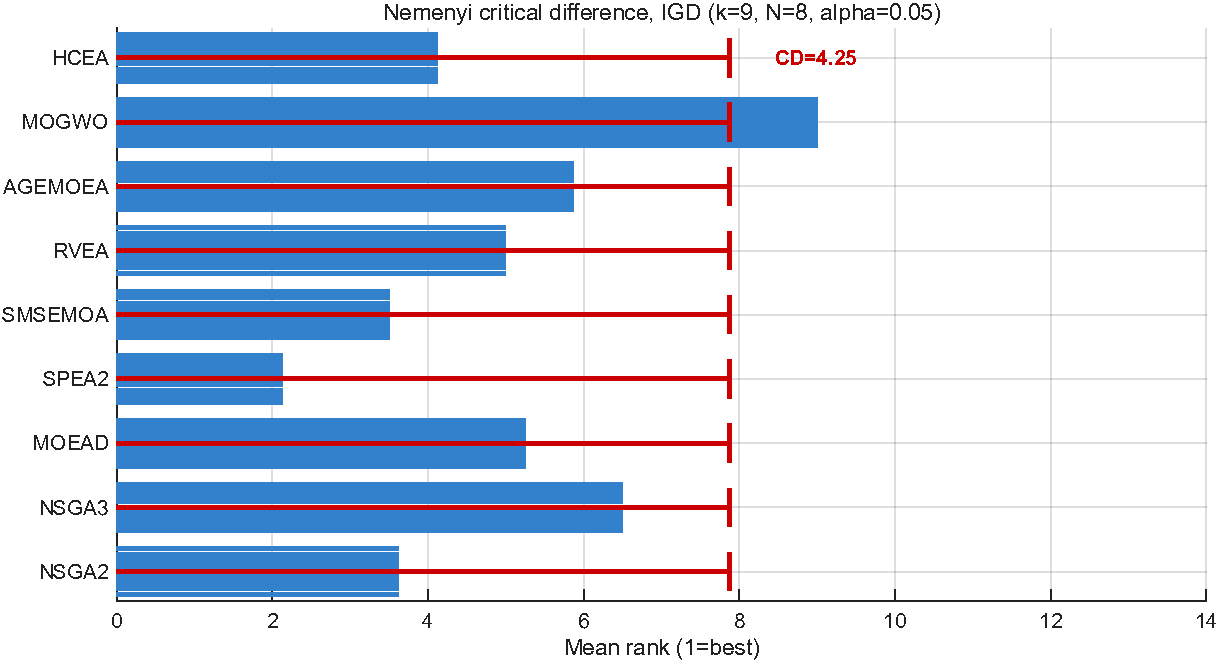
\includegraphics[width=0.48\columnwidth]{figures/fig4_cd_igd.pdf}}
\hfill
\subfloat[HV]{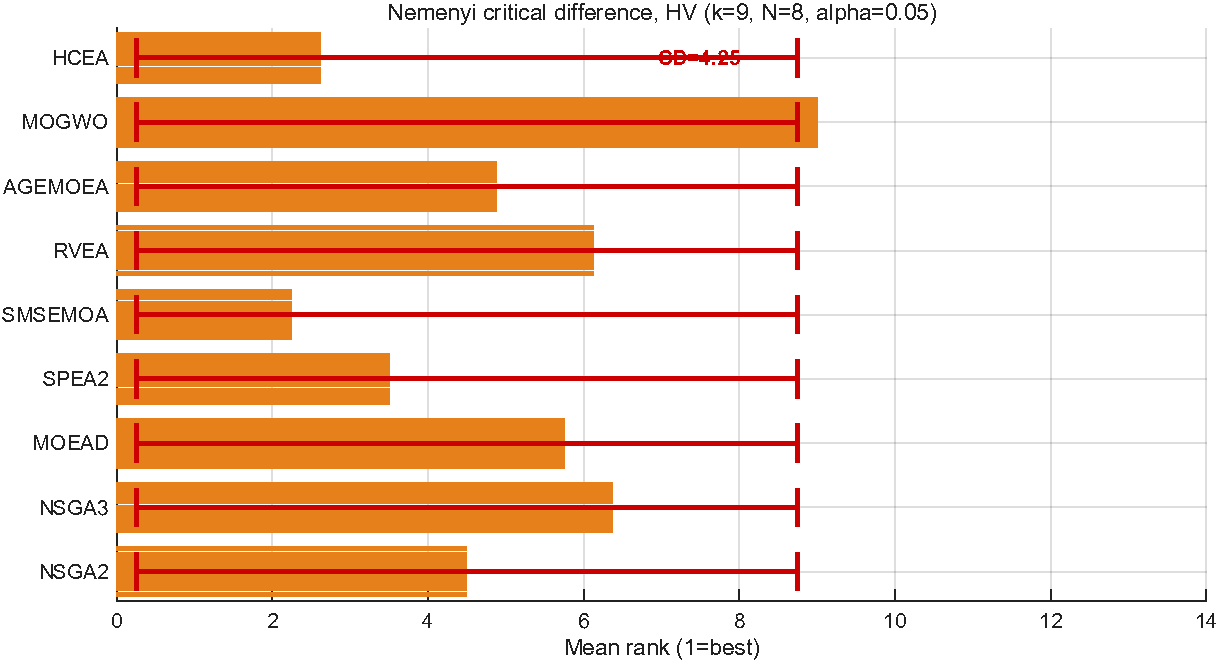
\includegraphics[width=0.48\columnwidth]{figures/fig4_cd_hv.pdf}}
\caption{Nemenyi critical-difference diagrams at $\alpha=0.05$ (k=9, N=5 blocks, CD=5.37). Algorithms connected by a horizontal bar are not significantly different.}
\label{fig:cd}
\end{figure}

\subsection{Indicator disagreement on concave fronts}
Figure~\ref{fig:boxplots} shows the 30-seed IGD distributions; Table~\ref{tab:ranks} makes the DTLZ2 divergence explicit: SMS-EMOA and HCEA occupy HV ranks 1--2 and IGD ranks 5--6, while MOEA/D and RVEA occupy IGD ranks 1 and 3 and HV ranks 4 and 6. The follow-up analysis (recomputing IGD on the same saved solution sets against an arc-uniform reference front) yields $\rho=0.63$ versus $0.57$ for the NBI-discretized front, ruling out reference-front discretization as the cause. [TODO: formalize this follow-up as a table or appendix.]

\begin{figure}[t]
\centering
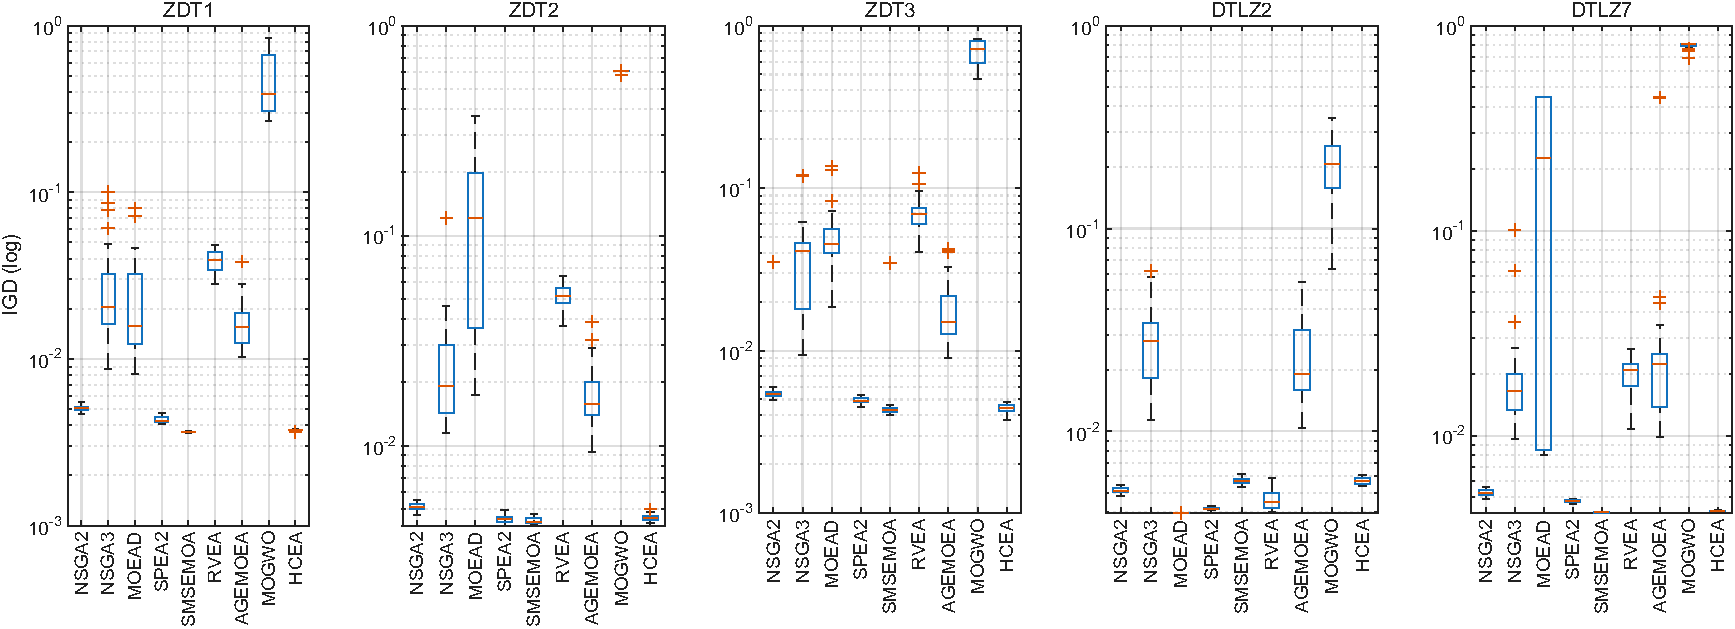
\includegraphics[width=\columnwidth]{figures/fig5_boxplots_5problems.pdf}
\caption{IGD distributions over 30 seeds for the five problems (log scale).}
\label{fig:boxplots}
\end{figure}

\begin{table}[t]
\centering
\caption{Total wall-clock time over the full study (8 problems $\times$ 30 seeds = 240 runs per algorithm) and mean number of function evaluations per run.}
\label{tab:runtime}
\begin{tabular}{lccc}
\toprule
Algorithm & Total time (s) & Mean nFE per run & maxGen \\
\midrule
NSGA2 & 23.0 & 20100 & 200 \\
NSGA3 & 67.0 & 20100 & 200 \\
MOEAD & 229.2 & 20100 & 200 \\
SPEA2 & 282.7 & 20100 & 200 \\
SMSEMOA & 1170.6 & 20100 & 200 \\
RVEA & 49.1 & 20100 & 200 \\
AGEMOEA & 390.4 & 20100 & 200 \\
MOGWO & $\approx$621 & 20100 & 200 \\
HCEA & 371.1 & 20191 & 200 \\
\midrule
\multicolumn{4}{l}{\footnotesize Note: all algorithms used maxGen = 200. MOGWO time is the sum of the M3 runs (1406\,s, from m3\_raw\_data.mat) and the 200-generation M2 runs (elapsed time not stored in mogwo\_200gen.mat; estimated $\approx$215\,s).}\\
\bottomrule
\end{tabular}
\end{table}


\section{Discussion}
The DTLZ2 divergence has a geometric explanation: HV-optimal placements on a concave front cluster toward the middle of the arc where the dominated boxes are largest, whereas IGD rewards arc-uniform coverage. Consequently, algorithm rankings on concave fronts are indicator-dependent, and claims that one algorithm dominates another must state the indicator. For HCEA specifically, the switch is hypervolume-verified, so its DTLZ2 behavior (switch accepted, HV rank 2, IGD rank 6) is the expected---and honest---outcome of maximizing its design criterion. [TODO: discuss which indicator suits which decision-making context; ablations of HCEA components (tournament vs. random mating, HV top-N vs. incremental reduction, static vs. adaptive reference vectors) as a table.]

\section{Conclusion}
We quantified IGD--HV ranking disagreement across five front geometries and showed that it concentrates on concave fronts and is not caused by reference-front discretization. We proposed HCEA, whose hypervolume-verified mechanism switch yields a top-tier algorithm: best on the disconnected ZDT3 in both metrics, Friedman HV rank 1.8, and no significant difference from SMS-EMOA and SPEA2 on most problems; its DTLZ2 IGD rank of 6 is reported as a genuine weakness. Future work extends HCEA to three or more objectives (where HV requires Monte Carlo estimation), constrained problems, and a wider sensitivity study of the checkpoint schedule. [TODO: final polish once all tables/figures are final.]

\section*{Acknowledgment}
[TODO: funding and acknowledgment.]

% \bibliographystyle{IEEEtran}
% \bibliography{references}

\begin{thebibliography}{1}
\bibitem{deb2002nsga2} K.~Deb, A.~Pratap, S.~Agarwal, and T.~Meyarivan, ``A fast and elitist multiobjective genetic algorithm: NSGA-II,'' \emph{IEEE Trans. Evol. Comput.}, vol.~6, no.~2, pp.~182--197, 2002.
\bibitem{zitzler2001spea2} E.~Zitzler, M.~Laumanns, and L.~Thiele, ``SPEA2: Improving the strength Pareto evolutionary algorithm,'' TIK-Report 103, ETH Zurich, 2001.
\bibitem{zhang2007moead} Q.~Zhang and H.~Li, ``MOEA/D: A multiobjective evolutionary algorithm based on decomposition,'' \emph{IEEE Trans. Evol. Comput.}, vol.~11, no.~6, pp.~712--731, 2007.
\bibitem{deb2014nsga3} K.~Deb and H.~Jain, ``An evolutionary many-objective optimization algorithm using reference-point-based nondominated sorting approach, Part I,'' \emph{IEEE Trans. Evol. Comput.}, vol.~18, no.~4, pp.~577--601, 2014.
\bibitem{cheng2016rvea} R.~Cheng, Y.~Jin, M.~Olhofer, and B.~Sendhoff, ``A reference vector guided evolutionary algorithm for many-objective optimization,'' \emph{IEEE Trans. Evol. Comput.}, vol.~20, no.~5, pp.~773--791, 2016.
\bibitem{beume2007smsemoa} N.~Beume, B.~Naujoks, and M.~Emmerich, ``SMS-EMOA: Multiobjective selection based on dominated hypervolume,'' \emph{Eur. J. Oper. Res.}, vol.~181, no.~3, pp.~1653--1669, 2007.
\bibitem{mirjalili2016mogwo} S.~Mirjalili, S.~Saremi, S.~M.~Mirjalili, and L.~S.~Coelho, ``Multi-objective grey wolf optimizer: A novel algorithm for multi-criterion optimization,'' \emph{Expert Syst. Appl.}, vol.~47, pp.~106--119, 2016.
\bibitem{li2014frrmab} K.~Li, \'A.~Fialho, S.~Kwong, and Q.~Zhang, ``Adaptive operator selection with bandits for a multiobjective evolutionary algorithm based on decomposition,'' \emph{IEEE Trans. Evol. Comput.}, vol.~18, no.~1, pp.~114--130, 2014.
\bibitem{zitzler2003performance} E.~Zitzler, L.~Thiele, M.~Laumanns, C.~M.~Fonseca, and V.~G.~da~Fonseca, ``Performance assessment of multiobjective optimizers: An analysis and review,'' \emph{IEEE Trans. Evol. Comput.}, vol.~7, no.~2, pp.~117--132, 2003.
\end{thebibliography}

\end{document}
